\documentclass[12pt]{article}
\usepackage[left=0.25cm,top=1cm,right=0.25cm,bottom=1cm]{geometry}
\textwidth = 20cm
\hoffset = -1cm
\usepackage[utf8]{inputenc}
\usepackage[spanish,es-tabla]{babel}
\usepackage[autostyle,spanish=mexican]{csquotes}
\usepackage[tbtags]{amsmath}
\usepackage{nccmath}
\usepackage{amsthm}
\usepackage{amssymb}
\usepackage{graphicx}
\usepackage{standalone}
\usepackage[outdir=./]{epstopdf}
\usepackage{siunitx}
\usepackage{physics}
\usepackage{color}
\usepackage{float}
\usepackage{multicol}
%\usepackage{milista}
\usepackage{enumitem}
\usepackage{anyfontsize}
\usepackage{anysize}
\usepackage{enumitem}
\usepackage{capt-of}
\usepackage{bm}
\usepackage{relsize}
\usepackage{placeins}
\usepackage{empheq}
\usepackage{cancel}
\usepackage{wrapfig}
\spanishdecimal{.}
\renewcommand{\baselinestretch}{1.5} 
\renewcommand\labelenumii{\theenumi.{\arabic{enumii}}}
\newcommand{\ptilde}[1]{\ensuremath{{#1}^{\prime}}}
\newcommand{\stilde}[1]{\ensuremath{{#1}^{\prime \prime}}}
\newcommand{\ttilde}[1]{\ensuremath{{#1}^{\prime \prime \prime}}}
\newcommand{\ntilde}[2]{\ensuremath{{#1}^{(#2)}}}


\usepackage{apacite}
\title{Examen - Tarea 4 \\[0.3em]  \large{Matemáticas Avanzadas de la Física}\vspace{-3ex}}
\author{M. en C. Gustavo Contreras Mayén}
\date{ }
\begin{document}
\vspace{-4cm}
\maketitle
\fontsize{14}{14}\selectfont

\textbf{Indicaciones: } Deberás de resolver cada ejercicio de la manera más completa, ordenada y clara posible, anotando cada paso así como las operaciones involucradas. El puntaje de cada ejercicio es de \textbf{1 punto}, excepto en donde se indica.

\begin{enumerate}
%Ref. Farrell IV-10
\item \textbf{(2 puntos) } Si la temperatura $T$ en la superficie de una esfera sólida de radio $R$ con centro en el origen, se mantiene a $T_{0} \, (1 - \cos \phi)$, donde $T_{0}$ es una constante y $\phi$ es el ángulo de colatitud desde el eje positivo $z$ en coordenadas esféricas. Determina la distribución de temperatura en estado estacionario en el sólido.
\item \textbf{(2 puntos) } Una esfera conductora de calor de radio $a$ está compuesta por dos hemisferios con un espacio infinitesimal aislante entre ellos, como se muestra en la figura (\ref{fig:figura2}). Las mitades superior e inferior de la esfera están en contacto con baños térmicos de temperaturas $+ T_{1}$ y $-T_{1}$, respectivamente. La esfera de radio $a$ está dentro de otra esfera conductora de calor de radio $b$ con una temperatura $T_{2}$.
\begin{figure}[H]
    \centering
   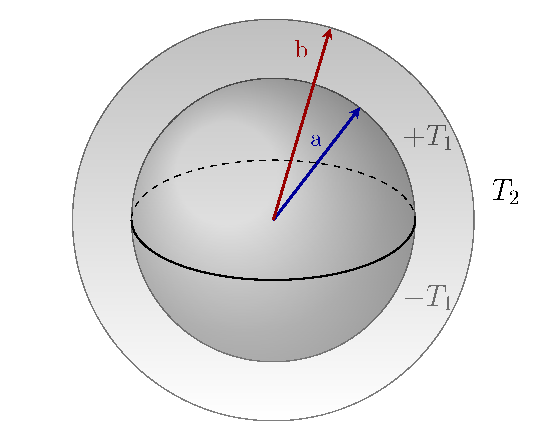
\includegraphics[scale=0.8]{Imagenes/esfera1.eps}
    \caption{Los hemisferios de la esfera interior se encuentran a diferentes temperatura.}
    \label{fig:figura2}
\end{figure}
Calcula la temperatura en los puntos:
\begin{enumerate}
\item Dentro de la esfera interior,
\item En la región entre las dos esferas y
\item Por fuera de la esfera exterior.
\end{enumerate} 
\item \textbf{(2 puntos) } En la figura (\ref{fig:esfera_aterrizada}) se muestra una esfera de radio $a$ con un pequeño espacio aislante en su ecuador, el hemisferio se encuentra aterrrizado, mientras que hemisferio superior se mantiene a un potencial constante $V_{0}$. 
\begin{figure}[H]
    \centering
   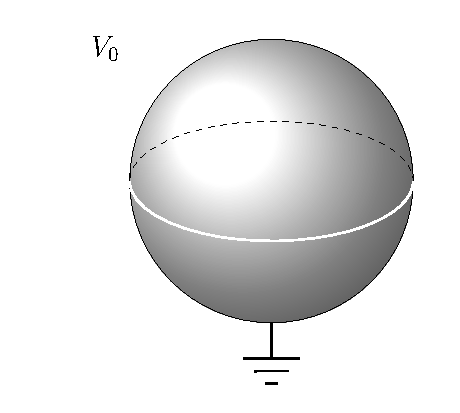
\includegraphics[scale=0.8]{Imagenes/esfera_5.eps}
    \caption{El hemisferio inferior se encuentra aterrizado.}
    \label{fig:esfera_aterrizada}
\end{figure}
Calcula el potencial electrostático en puntos dentro de la esfera.
%Ref. Arfken 12.3.11
\item \textbf{(1 punto) } La amplitud de una onda dispersada está dada por:
\begin{align*}
f(\theta) = \dfrac{1}{k} \, \nsum_{l = 0}^{\infty} (2 \, l + 1) \, \exp(i \, \delta_{l}) \, \sin \delta_{l} \, P_{l} (\cos \theta)
\end{align*}
Donde $\theta$ es el ángulo de dispersión, $l$ es el valor propio del momento angular, $\hbar \, k$ es el momento incidente, y $\delta_{l}$ es el desplazamiento de fase producido por el potencial central que está haciendo la dispersión. La sección transversal total es:
\begin{align*}
\sigma_{\text{tot}} = \scaleint{6ex} \abs{f(\theta)}^{2} \dd{\Omega}
\end{align*}
Demuestra que:
\begin{align*}
\sigma_{\text{tot}} = \dfrac{4 \, \pi}{k^{2}} \nsum_{l=0}^{\infty} (2 \, l + 1) \, \sin^{2} \delta_{l}
\end{align*}
%Ref. Arfken 12.5.7
\item \textbf{(1 punto) } Demuestra que:
\begin{align*}
\sin \theta \, \dv{\cos \theta} \, P_{n} (\cos \theta) = P_{n}^{1} (\cos \theta)
\end{align*}
%Ref. Arfken 12.5.10
\item \textbf{(1 punto) } Evalúa la siguiente integral:
\begin{align*}
\scaleint{5ex}_{\bs 0}^{2 \pi} \sin^{2} \theta \, P_{n}^{1} (\cos \theta) \dd{\theta}
\end{align*}
%Ref. Arfken 12.6.6
\item \textbf{(1 punto) } Recupera la relación de completitud (\emph{de cerradura o completes}) de los armónicos esféricos:
\begin{align*}
\nsum_{l=0}^{\infty} \nsum_{m=-l}^{l} Y_{l}^{m} (\theta_{1}, \varphi_{1})^{*} \, Y_{l}^{m} (\theta_{2}, \varphi_{2}) &= \dfrac{1}{\sin \theta_{1}} \, \delta(\theta_{1} - \theta_{2}) \, \delta (\varphi_{1} - \varphi_{2}) \\[0.5em]
&= \delta(\cos \theta_{1} - \cos \theta_{2}) \, \delta (\varphi_{1} - \varphi_{2})
\end{align*}
\end{enumerate}




\end{document}